\documentclass[man]{apa6}

\usepackage{amssymb,amsmath}
\usepackage{ifxetex,ifluatex}
\usepackage{fixltx2e} % provides \textsubscript
\ifnum 0\ifxetex 1\fi\ifluatex 1\fi=0 % if pdftex
  \usepackage[T1]{fontenc}
  \usepackage[utf8]{inputenc}
\else % if luatex or xelatex
  \ifxetex
    \usepackage{mathspec}
    \usepackage{xltxtra,xunicode}
  \else
    \usepackage{fontspec}
  \fi
  \defaultfontfeatures{Mapping=tex-text,Scale=MatchLowercase}
  \newcommand{\euro}{€}
\fi
% use upquote if available, for straight quotes in verbatim environments
\IfFileExists{upquote.sty}{\usepackage{upquote}}{}
% use microtype if available
\IfFileExists{microtype.sty}{\usepackage{microtype}}{}

% Table formatting
\usepackage{longtable, booktabs}
\usepackage{lscape}
% \usepackage[counterclockwise]{rotating}   % Landscape page setup for large tables
\usepackage{multirow}		% Table styling
\usepackage{tabularx}		% Control Column width
\usepackage[flushleft]{threeparttable}	% Allows for three part tables with a specified notes section
\usepackage{threeparttablex}            % Lets threeparttable work with longtable

% Create new environments so endfloat can handle them
% \newenvironment{ltable}
%   {\begin{landscape}\begin{center}\begin{threeparttable}}
%   {\end{threeparttable}\end{center}\end{landscape}}

\newenvironment{lltable}
  {\begin{landscape}\begin{center}\begin{ThreePartTable}}
  {\end{ThreePartTable}\end{center}\end{landscape}}

  \usepackage{ifthen} % Only add declarations when endfloat package is loaded
  \ifthenelse{\equal{\string man}{\string man}}{%
   \DeclareDelayedFloatFlavor{ThreePartTable}{table} % Make endfloat play with longtable
   % \DeclareDelayedFloatFlavor{ltable}{table} % Make endfloat play with lscape
   \DeclareDelayedFloatFlavor{lltable}{table} % Make endfloat play with lscape & longtable
  }{}%



% The following enables adjusting longtable caption width to table width
% Solution found at http://golatex.de/longtable-mit-caption-so-breit-wie-die-tabelle-t15767.html
\makeatletter
\newcommand\LastLTentrywidth{1em}
\newlength\longtablewidth
\setlength{\longtablewidth}{1in}
\newcommand\getlongtablewidth{%
 \begingroup
  \ifcsname LT@\roman{LT@tables}\endcsname
  \global\longtablewidth=0pt
  \renewcommand\LT@entry[2]{\global\advance\longtablewidth by ##2\relax\gdef\LastLTentrywidth{##2}}%
  \@nameuse{LT@\roman{LT@tables}}%
  \fi
\endgroup}


  \usepackage{graphicx}
  \makeatletter
  \def\maxwidth{\ifdim\Gin@nat@width>\linewidth\linewidth\else\Gin@nat@width\fi}
  \def\maxheight{\ifdim\Gin@nat@height>\textheight\textheight\else\Gin@nat@height\fi}
  \makeatother
  % Scale images if necessary, so that they will not overflow the page
  % margins by default, and it is still possible to overwrite the defaults
  % using explicit options in \includegraphics[width, height, ...]{}
  \setkeys{Gin}{width=\maxwidth,height=\maxheight,keepaspectratio}
\ifxetex
  \usepackage[setpagesize=false, % page size defined by xetex
              unicode=false, % unicode breaks when used with xetex
              xetex]{hyperref}
\else
  \usepackage[unicode=true]{hyperref}
\fi
\hypersetup{breaklinks=true,
            pdfauthor={},
            pdftitle={Effects of perceptual training on Cantonese productions of English plosives},
            colorlinks=true,
            citecolor=blue,
            urlcolor=blue,
            linkcolor=black,
            pdfborder={0 0 0}}
\urlstyle{same}  % don't use monospace font for urls

\setlength{\parindent}{0pt}
%\setlength{\parskip}{0pt plus 0pt minus 0pt}

\setlength{\emergencystretch}{3em}  % prevent overfull lines


% Manuscript styling
\captionsetup{font=singlespacing,justification=justified}
\usepackage{csquotes}
\usepackage{upgreek}

 % Line numbering
  \usepackage{lineno}
  \linenumbers


\usepackage{tikz} % Variable definition to generate author note

% fix for \tightlist problem in pandoc 1.14
\providecommand{\tightlist}{%
  \setlength{\itemsep}{0pt}\setlength{\parskip}{0pt}}

% Essential manuscript parts
  \title{Effects of perceptual training on Cantonese productions of English
plosives}

  \shorttitle{L2 production of English plosives}


  \author{Ana N. Rinzler\textsuperscript{1}}

  % \def\affdep{{""}}%
  % \def\affcity{{""}}%

  \affiliation{
    \vspace{0.5cm}
          \textsuperscript{1} Rutgers University, the State University of New Jersey\\
          \textsuperscript{}   }

  \authornote{
    Cognitive Psychology
    
    The Center for Cognitive Science
    
    I would like to thank Dr.~Terry Kit-fong Au from the University of Hong
    Kong for permitting us to conduct acoustic analyses on production data
    from her research.
    
    Correspondence concerning this article should be addressed to Ana N.
    Rinzler, 1498 State Rte. 28 West Hurley, NY 12491. E-mail:
    \href{mailto:anb136@psych.rutgers.edu}{\nolinkurl{anb136@psych.rutgers.edu}}
  }


  



  \usepackage{tipa}

\usepackage{amsthm}
\newtheorem{theorem}{Theorem}[section]
\newtheorem{lemma}{Lemma}[section]
\theoremstyle{definition}
\newtheorem{definition}{Definition}[section]
\newtheorem{corollary}{Corollary}[section]
\newtheorem{proposition}{Proposition}[section]
\theoremstyle{definition}
\newtheorem{example}{Example}[section]
\theoremstyle{definition}
\newtheorem{exercise}{Exercise}[section]
\theoremstyle{remark}
\newtheorem*{remark}{Remark}
\newtheorem*{solution}{Solution}
\begin{document}

\maketitle

\setcounter{secnumdepth}{0}



\section{Methods}\label{methods}

In this study, acoustic analyses were conducted on Cantonese speakers'
productions of English phonological minimal word pairs with voiced (i.e.
/b d g/) and voiceless (i.e. /p t k/) plosives in coda position. The
production of the word \enquote{got} was excluded from these analyses as
it was the only word that did not have a minimal pair. For all other
productions, PRAAT was used to measure the duration of the vowel.
Measuring vowel duration was motivated by evidence that vowel length is
an acoustic cue that English speakers use when distinguishing between
the following plosive as voiced or voiceless. For instance, the duration
of the vowel preceding a voiced plosive is typically longer than the
duration of a vowel preceding a voiceless plosive (House and Fairbanks,
1953; Peterson and Lehiste, 1960; House, 1961; Umeda, 1975; Klatt,
1976). Please note that the production data analyzed in this study was
collected and generously provided by Dr.~Terry Kit-fong Au, from the
University of Hong Kong.

\subsection{Participants}\label{participants}

There were a total of 36 undergraduate students from the University of
Hong Kong. 18 of the participants were in the training group (33\% men),
and 18 of the participants were in a wait-list control group (28\% men).

\subsection{Material}\label{material}

The following analyses are based on productions of phonological minimal
word pairs with voiced and voiceless plosives in coda position. The
vowel duration from the following words with a voiced coda were
analyzed:/b\ae d, bæg, k\ae b, k\textturnv b , d\textopeno g , f\ae d,
fid, p\textsci g, t\ae b/. The following words with a voiceless coda
were analyzed: / b\ae t, b\ae k, k\ae p, k\textturnv p, d\textscripta k,
f\ae t, fit, p\textsci k, t\ae b/. Only post-training productions were
examined in this study. For the wait-list control participants, these
productions represent the second time that participants produced the
minimal pairs. In other words, they did not receive training in between
the first time and second time that they produced these words.
Conversely, for trained participants, these productions represent the
second time that they produced these minimal pairs after receiving
training.

\subsection{Procedure}\label{procedure}

Participants in Au's (ms) study completed a 4 - 6 week training program
compromised of comprehending and producing English phonological minimal
word pairs. The purpose of training was to improve Cantonese speaker's
ability to perceive and produce notoriously difficult English contrasts.
The data analyzed in this study are words in which the contrast occurs
in coda position. The productions were then sent to our lab for acoustic
analyses.

The software PRAAT was used to conduct acoustic analyses. Textgrids were
created from the .wav sound files in order to mark the beginning and end
of the vowel boundary. Utilizing Sennheiser HD 555 headphones, the
beginning of the vowel was marked using the \emph{wav} method and the
end of the vowel was marked using the \emph{F2} method. All boundaries
were marked at the zero-crossing line. Measurements at present, were
only taken by one researcher. Thus, future cross-validation through
concordance rates is required. PRAAT scripting was then used to export
vowel duration measurements.

\subsection{Data analysis}\label{data-analysis}

All analyses were conducted using R (R Core Team, 2012) and \emph{lme4}
(Bates, Maechler \& Bolker, 2012). See \emph{Footnotes} for complete
list of R packages used. Data from the production task were analyzed
using a general linear mixed-effects model. The criterion variable was
\emph{vowel duration} which was convereted to milliseconds and
normalized for speaker. There were two predictors which were fixed
factors: (1) training \emph{trained/untrained} and voicing (2)
\emph{voiced/voiceless}. Both factors were categorical and were sum
coded. For the training variable, \emph{trained} (i.e.~participants who
were trained) were assigned a 1, and \emph{untrained} (i.e.~participants
who were not trained) were assigned a 0; while \emph{voiced} (i.e.~words
with voiced plosives in coda position) were assigned a 1 and
\emph{voiceless} were assigned a 0 (i.e.~words with voiceless plosives
in coda position). Two new columns in the data frame were generated to
represent the sum variables of the training and the voicing conditions.
The variable participant was treated as a random effect as each
participant had multiple productions. In other words, each participant
produced all of the 36 voiced (18) and voiceless (18) words. Visual
inspection of the Q-Q plots and plots of residuals against fitted values
revealed no violations of normality or homoscedasticity. Lastly,
statistical significance of voicing and training, and the voicing by
training interaction was accessed using hierarchical portioning of
variance via nested model comparisons, with the voicing variable entered
first into all models. P-values were obtained using likelihood ratio
tests comparing all models against the null model, and the alpha level
was set a \emph{p} \textless{} .05.

\section{Results}\label{results}

The interaction model explained the most variance (marginal \(R^2\) of
.052; conditional \(R^2\) of .305) and thus was used to interpret the
data. The interaction model explained more variance than just voicing or
training alone. The model with only voicing had a marginal \(R^2\) of
.045, conditional \(R^2\) of .295; and the model with only training had
a marginal \(R^2\) of .003, and a conditional \(R^2\) of .253. It is
clear that training factor contributed the least to overall variance
explained. The interaction model, however revealed that there was a main
effect of \emph{voicing} {[}\(\chi^2\) (1)=44.664, \emph{p}
\textless{}.001{]}, but no main effect of \emph{training} {[}\(\chi^2\)
(1)=0.4302, \emph{p} =0.5119{]}. There was however, an interaction
between \emph{voicing} \emph{x} \emph{training} {[}\(\chi^2\)
(4)=40.342, \emph{p} \textless{}.05{]}. The intercept mean was 177.98
(ms). The effect of \emph{voicing} (t = 6.478, \emph{p} \textless{}
.001) on this intercept was 11.65 +/- resulting in a range of
\emph{voiced} plosives having a mean vowel duration of approximately
189.63 (ms) +/- 1.8 (se); while the mean vowel duration for
\emph{voiceless} plosives was approximately 166.34 (ms) +/- 1.8 (se).
However, this effect was modulated by the interaction between
\emph{voicing} and \emph{training} - although this effect just reached
significance (t = 1.978, \emph{p} = 0.048). When the interaction between
\emph{voicing} and \emph{training} was considered, the vowel duration
mean increased \emph{voiced} plosive duration to 193.19 (ms) +/- 4.805
(se) and \emph{voiceless} plosive duration to 162.78 (ms) +/- 4.805
(se). Visual inspection of the data in \emph{Figure 1.} below suggests
that vowel durations were longer for trained participants, however this
can not be concluded from sum coding directly. Multiple comparisons of
the means are required.

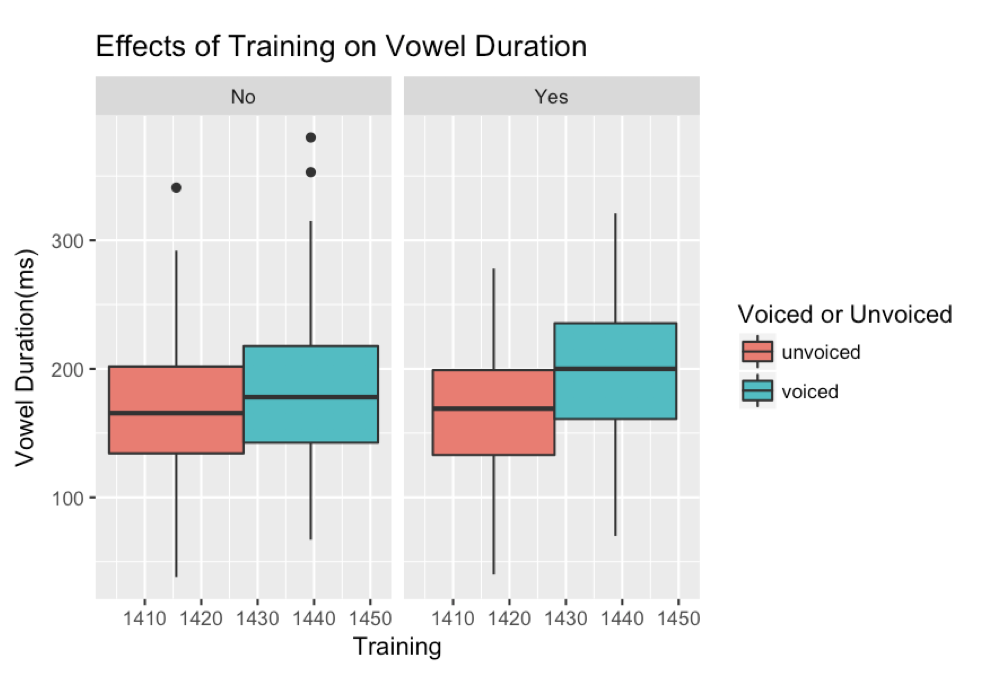
\includegraphics{/Users/anarinzler/Documents/GitHub/final_project/manuscript/figs/fig1}
\emph{Figure 1.} \emph{The above boxplot illustrates the differences in
vowel duration for trained and untrained participants for words with
voiced and voiceless plosives in coda position.}

\section{Discussion}\label{discussion}

Overall, the results suggest that participants produced words with
voiced plosives longer than words with voiceless plosives, and that this
effect was modulated by training. This suggests that vowel duration is
an acoustic cue that Cantonese speakers use when making the distinction
in English between words with voiced and voiceless plosives in coda
position. However, there was no main effect of training, so trained
participants did not differ significantly from untrained participants in
their productions of vowel duration.

Interestingly, there was an interaction between training and voicing.
This suggests that the factor \emph{training} may influence vowel
duration; at present it is unclear as to how this factor plays a role.
Graphical reprensentations of the data suggest that trained and
untrained participants had about equal vowel lengths for voiceless
plosives, and that trained participants had longer vowel durations for
voiced plosives, than untrained participants. This is in the direction
that I would predict, as trained participants received greater exposure
to instances of English productions.

The question then becomes: what is the nature of this exposure that
participants received? In other words, did the native English
productions contain vowels that had canconical and predictable vowel
durations, or was there extensive variation in the input they received?
It would not be surprising if participants received varying vowel
durations for two main reasons: (1) not all of the vowels in the minimal
pairs were identical (i.e.~d\textopeno g and d\textscripta k), and
furthermore some vowels are typically always longer in duration than
others (i.e.~f\ae d), and (2) the participants received input from four
different native English speakers. There is a debate as to whether
presenting listeners with input from multiple speakers has a positive or
negative effect on learnability. Regardless, it seems likely that
greater perceptual variability may obscure vowel duration as a cue, and
consequently diminish the probability of this utilizing this cue.

In future research, I plan to record monolingual English speakers
producing the minimal pairs from Au's (ms) study to measure their vowel
duration. I then plan to compare these durations to the Cantonese
speakers' productions in order to get a better idea of what native-like
vowel duration is. Additionally, I aim to explore other potential
acoustic cues that may be relevant for Cantonese speakers when making
these contrasts. For instance, I plan to measure aspiration duration,
mean aspiration intensity, F2 at the end of the vowel, as well as
closure duration. Aspiration is a phonological feature of Cantonese and
thus I predict it will play a role. Further, Cantonese is a tonal
language, and therefore F2 at the end of the vowel (a predictor of the
following plosive in English) may also be of interest.

\newpage

\section{References}\label{references}

\begingroup
\setlength{\parindent}{-0.5in} \setlength{\leftskip}{0.5in}

\hypertarget{refs}{}
\hypertarget{ref-R-papaja}{}
Aust, F., \& Barth, M. (2018). \emph{papaja: Create APA manuscripts with
R Markdown}. Retrieved from \url{https://github.com/crsh/papaja}

\hypertarget{ref-R-MuMIn}{}
Bartoń, K. (2018). \emph{MuMIn: Multi-model inference}. Retrieved from
\url{https://CRAN.R-project.org/package=MuMIn}

\hypertarget{ref-R-Matrix}{}
Bates, D., \& Maechler, M. (2018). \emph{Matrix: Sparse and dense matrix
classes and methods}. Retrieved from
\url{https://CRAN.R-project.org/package=Matrix}

\hypertarget{ref-R-lme4}{}
Bates, D., Mächler, M., Bolker, B., \& Walker, S. (2015). Fitting linear
mixed-effects models using lme4. \emph{Journal of Statistical Software},
\emph{67}(1), 1--48.
doi:\href{https://doi.org/10.18637/jss.v067.i01}{10.18637/jss.v067.i01}

\hypertarget{ref-R-purrr}{}
Henry, L., \& Wickham, H. (2017). \emph{Purrr: Functional programming
tools}. Retrieved from \url{https://CRAN.R-project.org/package=purrr}

\hypertarget{ref-R-doBy}{}
Højsgaard, S., \& Halekoh, U. (2018). \emph{DoBy: Groupwise statistics,
lsmeans, linear contrasts, utilities}. Retrieved from
\url{https://CRAN.R-project.org/package=doBy}

\hypertarget{ref-R-lmerTest}{}
Kuznetsova, A., Brockhoff, P. B., \& Christensen, R. H. B. (2017).
lmerTest package: Tests in linear mixed effects models. \emph{Journal of
Statistical Software}, \emph{82}(13), 1--26.
doi:\href{https://doi.org/10.18637/jss.v082.i13}{10.18637/jss.v082.i13}

\hypertarget{ref-R-likelihood}{}
Murphy, L. (2015). \emph{Likelihood: Methods for maximum likelihood
estimation}. Retrieved from
\url{https://CRAN.R-project.org/package=likelihood}

\hypertarget{ref-R-bindrcpp}{}
Müller, K. (2018). \emph{Bindrcpp: An 'rcpp' interface to active
bindings}. Retrieved from
\url{https://CRAN.R-project.org/package=bindrcpp}

\hypertarget{ref-R-tibble}{}
Müller, K., \& Wickham, H. (2018). \emph{Tibble: Simple data frames}.
Retrieved from \url{https://CRAN.R-project.org/package=tibble}

\hypertarget{ref-R-nlme}{}
Pinheiro, J., Bates, D., DebRoy, S., Sarkar, D., \& R Core Team. (2018).
\emph{nlme: Linear and nonlinear mixed effects models}. Retrieved from
\url{https://CRAN.R-project.org/package=nlme}

\hypertarget{ref-R-base}{}
R Core Team. (2017). \emph{R: A language and environment for statistical
computing}. Vienna, Austria: R Foundation for Statistical Computing.
Retrieved from \url{https://www.R-project.org/}

\hypertarget{ref-R-broom}{}
Robinson, D. (2018). \emph{Broom: Convert statistical analysis objects
into tidy data frames}. Retrieved from
\url{https://CRAN.R-project.org/package=broom}

\hypertarget{ref-R-ggfortify}{}
Tang, Y., Horikoshi, M., \& Li, W. (2016). Ggfortify: Unified interface
to visualize statistical result of popular r packages. \emph{The R
Journal}, \emph{8}(2). Retrieved from
\url{https://journal.r-project.org/}

\hypertarget{ref-R-ggplot2}{}
Wickham, H. (2009). \emph{Ggplot2: Elegant graphics for data analysis}.
Springer-Verlag New York. Retrieved from \url{http://ggplot2.org}

\hypertarget{ref-R-tidyverse}{}
Wickham, H. (2017). \emph{Tidyverse: Easily install and load the
'tidyverse'}. Retrieved from
\url{https://CRAN.R-project.org/package=tidyverse}

\hypertarget{ref-R-forcats}{}
Wickham, H. (2018a). \emph{Forcats: Tools for working with categorical
variables (factors)}. Retrieved from
\url{https://CRAN.R-project.org/package=forcats}

\hypertarget{ref-R-stringr}{}
Wickham, H. (2018b). \emph{Stringr: Simple, consistent wrappers for
common string operations}. Retrieved from
\url{https://CRAN.R-project.org/package=stringr}

\hypertarget{ref-R-tidyr}{}
Wickham, H., \& Henry, L. (2018). \emph{Tidyr: Easily tidy data with
'spread()' and 'gather()' functions}. Retrieved from
\url{https://CRAN.R-project.org/package=tidyr}

\hypertarget{ref-R-dplyr}{}
Wickham, H., Francois, R., Henry, L., \& Müller, K. (2017). \emph{Dplyr:
A grammar of data manipulation}. Retrieved from
\url{https://CRAN.R-project.org/package=dplyr}

\hypertarget{ref-R-readr}{}
Wickham, H., Hester, J., \& Francois, R. (2017). \emph{Readr: Read
rectangular text data}. Retrieved from
\url{https://CRAN.R-project.org/package=readr}

\hypertarget{ref-R-xaringan}{}
Xie, Y. (n.d.). \emph{Xaringan: Presentation ninja}. Retrieved from
\url{https://github.com/yihui/xaringan}

\hypertarget{ref-R-kableExtra}{}
Zhu, H. (2018). \emph{KableExtra: Construct complex table with 'kable'
and pipe syntax}. Retrieved from
\url{https://CRAN.R-project.org/package=kableExtra}

\endgroup

\newpage

\section{Footnotes}\label{footnotes}

\emph{The following lists the specific packages used in R:}

R (Version 3.4.3; R Core Team, 2017) and the R-packages \emph{bindrcpp}
(Version 0.2.2; Müller, 2018), \emph{broom} (Version 0.4.4; Robinson,
2018), \emph{doBy} (Version 4.6.1; Højsgaard \& Halekoh, 2018),
\emph{dplyr} (Version 0.7.4; Wickham, Francois, Henry, \& Müller, 2017),
\emph{forcats} (Version 0.3.0; Wickham, 2018a), \emph{ggfortify}
(Version 0.4.4; Tang, Horikoshi, \& Li, 2016), \emph{ggplot2} (Version
2.2.1; Wickham, 2009), \emph{kableExtra} (Version 0.8.0; Zhu, 2018),
\emph{likelihood} (Version 1.7; Murphy, 2015), \emph{lme4} (Version
1.1.17; Bates, Mächler, Bolker, \& Walker, 2015), \emph{lmerTest}
(Version 3.0.1; Kuznetsova, Brockhoff, \& Christensen, 2017),
\emph{Matrix} (Version 1.2.14; Bates \& Maechler, 2018), \emph{MuMIn}
(Version 1.40.4; Bartoń, 2018), \emph{nlme} (Version 3.1.137; Pinheiro,
Bates, DebRoy, Sarkar, \& R Core Team, 2018), \emph{papaja} (Version
0.1.0.9709; Aust \& Barth, 2018), \emph{purrr} (Version 0.2.4; Henry \&
Wickham, 2017), \emph{readr} (Version 1.1.1; Wickham, Hester, \&
Francois, 2017), \emph{stringr} (Version 1.3.0; Wickham, 2018b),
\emph{tibble} (Version 1.4.2; Müller \& Wickham, 2018), \emph{tidyr}
(Version 0.8.0; Wickham \& Henry, 2018), \emph{tidyverse} (Version
1.2.1; Wickham, 2017), and \emph{xaringan} (Version 0.6.4; Xie, n.d.)






\end{document}
